%% Before beginning to type your dissertation, read the formatting guide, 
%% which can be found at http://grad.msu.edu/etd/docs/formattingguide.pdf
%% Also get the latest version of msuphddissertation.cls and the template file
%% at http://www.math.msu.edu/~weil/MSU_Ph.D._Dissertation.zip
%% Send questions to weil@math.msu.edu
\documentclass{msuphddissertation_ssn}
%% Insert packages you wish to use except setspace and subfig. 
%% Those packages are loaded automatically.
%% IMPORTANT: Load only those packages you know you will use.
%% Some packages can cause conflicts resulting in improper formatting.
\usepackage[T1,T2A]{fontenc}
\usepackage[utf8]{inputenc}
\usepackage[english,russian]{babel}
\selectlanguage{english}
\usepackage{lipsum}
\usepackage{microtype}
\usepackage{graphicx}
\usepackage{caption}
\usepackage{setspace}
\usepackage{caption}
\captionsetup[table]{labelsep=space}
\captionsetup[figure]{labelsep=space}
\captionsetup[subfigure]{labelformat=parens,labelsep=space,font=small}
\usepackage{physics}
\usepackage[version=3]{mhchem} 
\usepackage{amsmath}
\usepackage{mathtools}
\usepackage{xfrac}
\usepackage{siunitx}
\usepackage{tikz}
\usepackage{cleveref}
\usepackage{import}
\usepackage{svg}



\author{Sarah Frechette Roberts} %% Put your name in full as it is officially recognized by Michigan State University here.
\title{Control of nitrogen related defects in doped single crystal diamond grown via chemical vapor deposition} %% Put the title of your dissertation here.
\unit{Material Science and Engineering - Doctor of Philosophy} %% 

%%%%%%%%%%%%%%%%%%%%%%%%%%%%
%%%%%%%% NOTE %%%%%%%%%%%%%%
%% PREPARING A DISSERTATION WITH THIS CLASS FILE DOES NOT %%%
%% GUARANTEE THAT THE GRADUATE SCHOOL WILL APPROVE IT %%%
%%%%%%%%%%%%%%%%%%%%%%%%%%%%%%%

%%%%%%%%%%%%%%%%%%%%%%%%%%%%%%%%%%
%%%%%%%%%%%% WARNING %%%%%%%%%%%%%%%
%% The Graduate School requires that all text, except superscripts %%
%% and subscripts, but including text in imported %%
%% graphics files be in 12 point. For that reason it's recommended %%
%% that no text be part of any imported files. %%

%% Once your document has been filed with the Graduate School,
%% if you wish to produce a version of it whose subscripts and superscripts
%% are in traditional smaller proportion, remove the "%" sign 
%% in front of following command. 
%\DeclareMathSizes{12}{12}{10}{8}
%% To single space your document, find and remove the 
%% two commands \begin{doublespace}
%% and \end{doublespace} below.

\begin{document}
\begin{otherlanguage}{english}
\maketitlepage %%This command will produce the title page of your thesis.
\begin{abstract}
\indent

Quantum sensing holds great potential for many intriguing applications such as vector magnetometry for magnetic field navigation in GPS disallowed scenarios and nanoscale magnetic resonance imaging (MRI). The negatively charged nitrogen vacancy defect (NV$^-$) in diamond is a promising candidate for quantum sensing applications. A key advantage of the NV$^−$ is its atomic size, which enables extraordinary spatial precision by single centers placed deterministically with minimal damage to the surrounding diamond lattice.  This has been accomplished with ultrafast laser writing, however the defect creation process, which creates vacancies in the diamond lattice with a femtosecond laser pulse and then diffuses them at lower laser power until they find single substitutional nitrogen atoms to form the NV\textsuperscript{−} centers, requires a very particular kind of substrate. The diamond lattice needs to contain sufficient substitutional nitrogen to allow for the NV\textsuperscript{−} formation but also needs to have a very low background of NV\textsuperscript{− }so that the written defects are single centers and distinguishable during the writing process. Furthermore, the high index of refraction of diamond causes the laser focal spot to be extended in the direction of the writing beam, and therefore the NV\textsuperscript{−} formation can occur far away from the surface where their sensitivity would be the highest. 

A materials engineering challenge, developing ideal laser writing substrates, aimed at improving resolution of quantum sensors through fabrication of arrays of single NV$^-$ centers was explored in this work. The ideal single crystal diamond (SCD) substrate contains a delta doped layer of single substitutional nitrogen to overcome the inaccuracy in depth placement, and very low NV$^-$ background. A parametric study of a bell jar style microwave plasma assisted chemical vapor deposition (CVD) reactor was performed to address this materials engineering challenge. The effects of substrate temperature, reactor pressure, substrate offcut, and substrate surface preparation on the incorporation of nitrogen related defects was determined using characterization techniques including Fourier-transform infrared spectroscopy (FTIR), Ultra-violet spectroscopy (UV-Vis), Raman spectroscopy, photoluminescent (PL) spectroscopy, Atomic Force Microscopy (AFM), Differential Interference Contrast Microscopy (DICM), and Electron Paramagnetic Resonance (EPR). Expansion of the operation region of the CVD reactor to a low growth rate regime was assessed to improve crystalline quality and reduce delta doped layer thickness. Finally, an investigation into surface preparation techniques was completed to normalize the substrate surface condition prior to deposition, ensuring quality growth and improving sensitivity of nitrogen incorporation due to deposition parameters.

This dissertation establishes a surface preparation method to normalize the substrate surface condition. Next, it validates growth quality in a low growth rate regime expanding the operation region of the CVD reactor. Lastly, the sensitivity of nitrogen incorporation caused by varying reactor parameters is investigated. These results elucidate the effectiveness of preparing laser writing substrates in the current bell jar style reactor and more broadly study the factors affecting nitrogen incorporation during CVD growth. 
	
\end{abstract}

%% If you wish to have a copyright page, remove the "%" in front of \begin{copyrt}
%% and remove the "%" in front of \end{copyrt}.
%% The mandatory form of the Copyright will be generated automatically. 
%% A copyright statement is optional.

%\begin{copyrt}
%\end{copyrt}

\begin{dedication} 
%put your dedication here
To the memory of Grandma Jan. I hope this achievement honors the legacy of success she dreamed of for her family. 
\end{dedication}

%% If you wish to have an acknowledgment, remove the "%" in front of \begin{acknowledgment}
%% and remove the "%" in front of \end{acknowledgment}
\begin{acknowledgment}
%% Type your acknowledgment here. An acknowledgment is optional.
\indent 

I would like to begin by expressing my deepest gratitude to my supervisor, Dr. Shannon Nicley, for her invaluable guidance, patience, and support throughout this process. Not only was her expertise in all aspects of synthetic diamond growth and insightful feedback instrumental in shaping this research and pushing me to become a better scholar, her perspectives and advice related to being a woman in STEM helped grow my confidence as a scientist and educator.

I am grateful my co-advisor, Dr. Jonas Becker, whose diamond in quantum technology knowledge and tough questions during group meetings helped me gain a deeper understanding of my research and its impacts. My committee members, Dr. Alexandra Zevalkink and Dr. Donald Morelli, deserve thanks for their time and the constructive critiques that helped refine my work. A special thanks to the faculty and staff in the Chemical Engineering and Materials Science department as well as the Electrical and Computer Engineering departments at Michigan State University for providing the resources and environment necessary to complete this thesis.

To my colleagues and peers in QuOD labs, thank you for the many hours of brainstorming, technical help, and most importantly the comedic relief. I would specifically like to thank Alex Loomis for his help with sample characterization and fruitful conversations about work and life; Kai Klink for their help with PL and confocal data collection and being a great study partner for quantum mechanics; Ian Morris, Andrew Kirkpatrick, and Logan Crooks for help with confocal microscopy and optics lab troubleshooting; Milos Sretenovic his attention to detail encouraging me to strive for the utmost quality; Theresa Alberth, Ethan Egger, and Nathan Jansen for all their support.

Fraunhofer Center Midwest CMW was foundational to my research success. I am thankful to the organization as a whole for providing access to essential data and resources. I am exceptionally grateful to Nina Baule, Aaron Hardy, Robert Rechenberg, Matthias Muehle, Luke Suter, Alex Ho, and Karl Dersch.

I started my research under the supervision of Dr. Elias Garratt whom I would like to extend my appreciation for his support in the early stages of research and connecting me with so many wonderful researchers. Shengyan Bai, thank you for teaching me the nuances of growing diamond in DS4. I could not have done this without your help. Additional thanks goes out to Erik Vyhmeister and Ramon Diaz for sharing their expertise. 

I am deeply indebted to all of my friends for their endless support. Christina, thank you not only for being the cheese to my curd throughout undergrad, but also for pushing me to take on the challenge of a PhD. I, legitimately, would not be here with you. To Chris, Kyra, Samantha, Nathan, Ryan, Alex, and Meghan for always being a constant source of support, perspective, and much needed distractions when things felt overwhelming.

Finally, I want to thank my family their unwavering belief in me. To my sister, Emily, thank you for your lifelong encouragement. Following in your footsteps wasn't always easy, but navigating new terrain knowing you were standing behind me every step of the way was. To my parents, Tommy and Angel, my brothers, Ben and Andrew, and my in-laws, Becky, Tom, and Ryan, and the rest of the amazing family I am so fortunate to have for the relentless support. Also, to my dog, Louis, for bringing me gifts in the form of his slobbery toys while I was writing. Most importantly, I owe immeasurable appreciation to Sean for being my partner, my best friend, and my rock through the years. Thank you for sticking by me through the long nights and for keeping me grounded when things got difficult.

\end{acknowledgment}

%% If you wish to have a preface, remove the "%" in front of \begin{preface}
%% and remove the "%" in front of \end{preface}. The formatting of
%% a preface isn't specified.
%\begin{preface}
%% Type your preface here. A preface is optional.
%\end{preface}

\TOC %% This command produces the Table of Contents. DO NOT REMOVE!

%% If your document contains tables, remove the "%" in front of 
%% the following line.
%\LOT

%% If your document contains figures, remove the "%" in front of
%% the following line.
%\LOF

%% If any of your figures contain color, you must
%% include the following disclaimer in the caption of your first figure.
%% "For interpretation of the references to color in this and all other figures, 
%% the reader is referred to the electronic version of this thesis."

%%%% LIST OF SYMBOLS AND ABBREVIATIONS %%%%
%% Such a list is possible using the environment
%% abbreviationskey
%% here. The list will be included in the TOC as
%% KEY TO SYMBOLS AND ABBREVIATIONS
%% To change the name something else, remove the "%" 
%% from the next line and change "Desired Name" to your choice.
%\renewcommand{\keyname}{Desired Name}
%%%%%%%%%%

\newpage

\end{otherlanguage}
\begin{doublespace}


%% Put the body of your dissertation here. 
%% DO NOT include the bibliography
\selectlanguage{english}
\pagenumbering{arabic}

%%%%%%%%%% NESTING .TEX FILES %%%%%%%%%
%Use this command in the document body to insert the contents of another file named filename.tex; again this file should not contain any LATEX preamble. LATEX will start a new page before processing the material input from filename.tex. Make sure not to include the extension .tex in the filename, as this will stop the file from being input (the extension can optionally be included with input and import). It is not possible to nest include commands. Each file that gets \included has its own .aux file storing information of created labels and contents for the table of contents, list of figures, etc. You can use \includeonly with a comma separated list of file names (make sure that there are no leading or trailing spaces). If you do this LATEX will only process the files contained in that list. This can be used to enhance compilation speed if you're only working on a small part of a bigger document. Page numbers and cross references will however still work, as the .aux files of left out files will still be processed.
%\include{Chapters/ExampleChapter.tex} 

\include{Chapters/BkgAndIntro}
%\include{Chapters/ExampleChapter}
\include{Chapters/DiamondGrowth}
\include{Chapters/CharMethods}
\include{Chapters/SubstrateSurfacePreparation}
\chapter{Low Methane Growth Regime in High Growth Rate Reactor}
\label{chLowCH4}

\section{Experimental Methods}
\section{Methane Concentration Effects on Growth Rate}
\section{Formation of Unepitaxial Crystallites}
\section{Unitentional Nitrogen Incorporation}
\section{Post-Processing to Reduce Nitrogen Vacancy Center}
\subsection{High Pressure Annealing}
\subsection{High Temperature Hydrogen Enviornment to Passivate Nitrogen Vacancy Center}

\include{Chapters/PressureOffcutEffects}
\chapter{Conclusions}
\indent

The purpose of this work was to understand nitrogen doped chemical vapor deposition of diamond such that optimized conditions could be selected for a desired outcome. In this case, the desired outcome is an ideal substrate for laser writing of nitrogen vacancy (NV) defect arrays which consists of a high quality single crystal diamond plate with a delta doped layer of single substitutional nitrogen. With an ideal substrate, spatial control of NV centers via laser writing will be significantly improved thus improving the spatial resolution of quantum sensors. Determining optimized conditions included understanding the effects of substrate surface preparation on deposition quality, establishing growth quality in a low growth rate regime which expanded the growth operation region of DS4, and a parametric study of reactor parameter effects on nitrogen incorporation. A method to determine nitrogen concentration from FTIR was developed to evaluate deposition quality. A summary of each investigation and concluding remarks on the success of each investigation as well as proposed future direction of each work will be presented here.

\section{Quantification of High Concentration of Substitutional Nitrogen via Fourier Infrared Transform Spectroscopy}
\indent

An accurate, non-destructive method for determining substitutional nitrogen concentration as opposed NV$^-$ was needed to optimized deposition conditions for laser writing substrates. Present methods were either destructive, lacked specificity, or were optimized for low to moderate concentration of nitrogen. The method was developed using FTIR absorption spectra for diamond films grown via CVD with high gas phase concentration of nitrogen. The grown films contained numerous nitrogen-related defects. An accurate, non-destructive method for determining substitutional nitrogen concentration in nitrogen-rich diamond was developed by deconvoluting nitrogen-related IR absorption peaks to determine peak area. Through deconvolution, absorption peaks parameters can be more accurately determined in the presence of strain and other nitrogen-related defects. EPR was used to validate the new method.

\section{Substrate Surface Preparation}
\indent

Several methods for substrate surface preparation were evaluated in Chapter \ref{chSurfacePrep}. First, every substrate was required to have surface roughness of not more than 1 nm after mechanical polishing. Then, an extended hydrogen plasma etch was incrementally administered to a single substrate. Microscale surface features and nanoscale surface roughness were evaluated after each increment. The hydrogen plasma etch preferentially etched polishing damage and dislocations in the substrate. This increased the surface roughness of the sample, after an slight decrease in the first 15 minute etch increment, as the etch time progressed. The same experiment was performed on a second substrate with fewer etch steps. Again, the surface roughness increased as cumulative etch time increased. The increase in surface roughness was a result of increased etch pits with exposed crystalline facets. The removal of amorphous polishing damage and exposure of crystalline facets resulted in low strain grown films. Lastly, a reactive ion etch was performed on the same starting substrate as the first hydrogen etch experiment, however, the grown film was removed and the surface was mechanically polished to not more than 1 nm surface roughness. The reactive ion etch ballistically removed 6.5 $\mu m$ of polishing damaged material from the center of the diamond substrate exposing clean single crystal diamond. The reactive ion etch preferentially etch the polishing lines, but exposed a smooth, low roughness, diamond surface. The reactive ion etch also produced a low strain high quality single crystal diamond film. The extended hydrogen plasma etch was implemented as the surface normalization process due to its ease of access during chemical vapor deposition of diamond, however, reactive ion etching demonstrated equivalent success in surface normalization.

\section{Low Methane Depositions}
\indent

Manufacturing of layered structures through CVD growth potentially requires the ability to slow down or halt growth rates during the deposition for changes in feed gas composition. The reactor used for the work presented in this dissertation was optimized for high growth rates of large single crystal diamond wafers. An experimental deposition series to expand the growth regime of the reactor was completed and high quality SCD growth was validated at the low growth rate conditions. Three samples at 3\%, 2\%, and 1\% methane with no intentional nitrogen doping were grown. Step flow growth, an indicator of high quality growth, was observed in all three depositions. Unepitaxial crystallites formed on the 1\% methane deposition indicating faster growth propagation from nucleation sites than overall vertical growth rate. In other words, the overall vertical plane growth rate did not outpace the growth of adatom nucleation site from early in the deposition process.

In addition to growth morphology, NV background was measured using photoluminescent spectroscopy. Each spectra was normalized to the Raman line allowing for qualitative comparison of intensities. As the methane concentration decreased, the NV concentration increased. This is due to the increased effect of non-negligible atmospheric leak rate into the reactor which increases the ratio of nitrogen to carbon as the methan concentration is decreased, allowing more nitrogen to incorporate in the SCD growth.

The high NV background at reduced growth rates defeats the purpose of utilizing slow growth rates to exchange feed gases and improve resolution of layered structures by minimizing transition layer thickness. The high growth rate reactor is therefore inadequate for layered structure growths due to large residence times and atmospheric nitrogen leak rate. Preliminary investigations into post-processing steps, including low pressure annealing and exposure to a high temperature hydrogen environment, did not reduce NV background of low methane depositions to a usable level for laser writing. 

\section{Effects of Pressure and Offcut on Nitrogen Incorporation}
\indent

A diamond substrate with a sufficient concentration of substitutional nitrogen and low background of NV$^-$ centers is necessary for deterministic laser writing arrays of single NV$^-$ centers. To preferentially incorporate nitrogen as substitutional nitrogen, a parametric study of reactor parameters was conducted to identify deposition conditions to suppress the incorporation of nitrogen as NV$^-$ and favor the incorporation of nitrogen as substitutional nitrogen. Deposition parameters evaluated include substrate temperature, reactor pressure, and substrate offcut. The first experimental series emphasized a correlation in nitrogen incorporation and the confounding variable of surface roughness.

The confounding variable of surface roughness was mitigated through a surface normalization procedure developed in Chapter \ref{chSurfacePrep}. The surface normalization procedure consisted of a mechanical polish of not more than 1 nm surface roughness followed by a 5 hour hydrogen plasma etch immediately prior to deposition. The second experimental series showed no correlation between nitrogen related defect incorporation and surface roughness indicating an effective surface normalization procedure.

Using the second experimental series with normalized surface condition, the effects of reactor pressure and substrate offcut on nitrogen incorporation were investigated. A high nitrogen concentration in the gas phase of the deposition was used to exaggerate the effects of deposition parameter variation on nitrogen incorporation. At high nitrogen concentrations, the sensitivity of reactor pressure and substrate surface orientation was too low to favor the incorporation of nitrogen as substitutional nitrogen and suppress the incorporation of nitrogen as NV$^-$. The NV$^-$ background of the surface normalized deposition series was too high for laser writing. This necessitates the exploration of reactor parameters with higher sensitivity.

The resolution of quantum sensors with NV$^-$ defects can be improved through addressing materials engineering challenges through creation of ideal substrates for laser writing. The manufacturing of these substrates requires precise control of gas phase composition to minimize transition layer thickness of a delta doped region. Further control of nitrogen defect selectivity within the delta doped layer is necessary to reduce NV$^-$ background and incorporation of single substitutional nitrogen.

\section{Proposed Future Work}
\indent
 
The conclusions of this work are that the current CVD reactor, DS4, is not suitable for creating delta doped layers, due to long residence times, high growth rate, and unitentional nitrogen concentration. A different reactor design, such as the NIRIM style reactor, would be better suited for delta doping due to the laminar flow rate of deposition gases. 

Reactor pressure and substrate offcut exhibited low sensitivity with respect to nitrogen defect selection at high gas phase nitrogen concentration. Exploration of other deposition parameters with higher sensitivity in needed. Potential deposition parameters include: low gas phase nitrogen concentration or different nitrogen sources.

Lastly, accurate characterization of nitrogen related defects through FTIR is valuable to non-destructive determination of single substitutional nitrogen concentration. The method developed deconvolutes a complicated absorption band in FTIR using seven Gaussian peaks and was validated using EPR spectroscopy. To ensure the seven nitrogen related peaks used for the fit are present, FTIR data can be taken at low temperatures to reduce the thermal broadening of the peaks allowing each peak to be more easily resolved. For this, a low temperature attachment for the FTIR is necessary.

This continued work would improve the quality of single crystal diamond laser writing substrates with a delta doped substitutional nitrogen layer. The improvement of the laser writing substrate will improve the resolution of NV$^-$ based quantum sensors.


%%%%%%% APPENDICES %%%%%%%%%%
%% If you wish to include one appendix, remove the "%" from the 
%% following two lines.
\renewcommand{\appname}{APPENDIX}
\appendix
%The next six (6) lines are here because we only have on appendix. This removes the trailing label "A" which is unecessary since there is only one appendix for the TOC entry. Added by Sarah July 23, 2026
\makeatletter
\renewcommand{\thechapter}{A} 
\setcounter{chapter}{1} 
\renewcommand{\chaptername}{Appendix} 
\renewcommand{\thechapter}{} 
\makeatother

\chapter{Naming Convention for Diamond Samples}
\label{SampleTracking}

%The next four (4) lines allows reinstitutes the trailing "A" now that the title of the chapter has printed. It allows for tables and figures to be labeled A.1, A.2, etc. Added by Sarah July, 23, 2026
\renewcommand{\thechapter}{A}
\setcounter{figure}{0}
\setcounter{table}{0}
\makeatother

\indent

The first step in characterizing diamond samples is naming the sample. As samples go through several changes, sample names need to be informative and modifiable such that origination and process history is preserved. A three part naming convention was developed. The naming convention starts with a source code which indicates the supplier or growth reactor, see Figure \ref{fig:nameSource}. The second part of the naming convention is the acquisition code which indicates the year the sample was acquired and the sequential order the sample was received within that year, see Figure \ref{fig:nameAcq}. The last part of the naming convention is the modification code which add or increments an alphabetical character for processing that modifies the bulk material properties. The modification code for surface treatments is a numeric character that should be added or incremented for subsequent surface treatments, see Figure \ref{fig:nameMod}. A graphical example of the implementation of this naming convention is show in Figure \ref{fig:nameEx}.

\begin{figure}
    \centering
    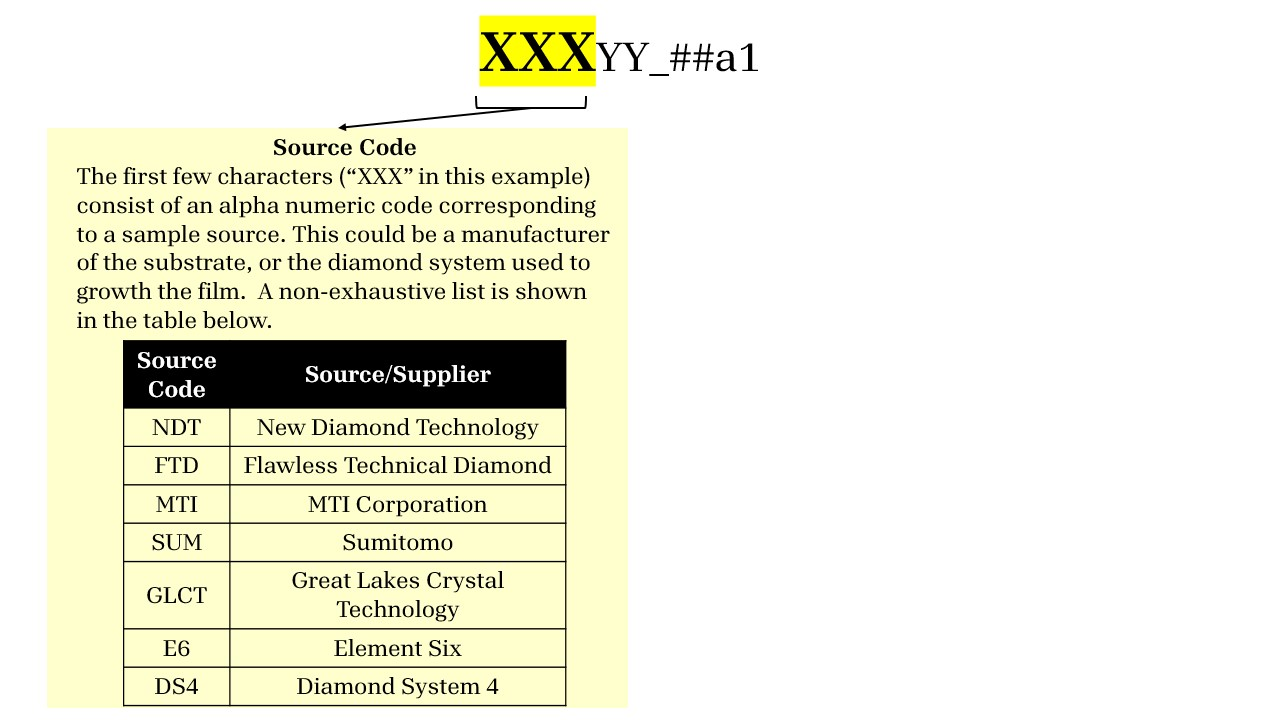
\includegraphics[width=1\linewidth]{figures/Slide2.jpg}
    \caption{Source code description for sample naming convention.}
    \label{fig:nameSource}
\end{figure}

\begin{figure}
    \centering
    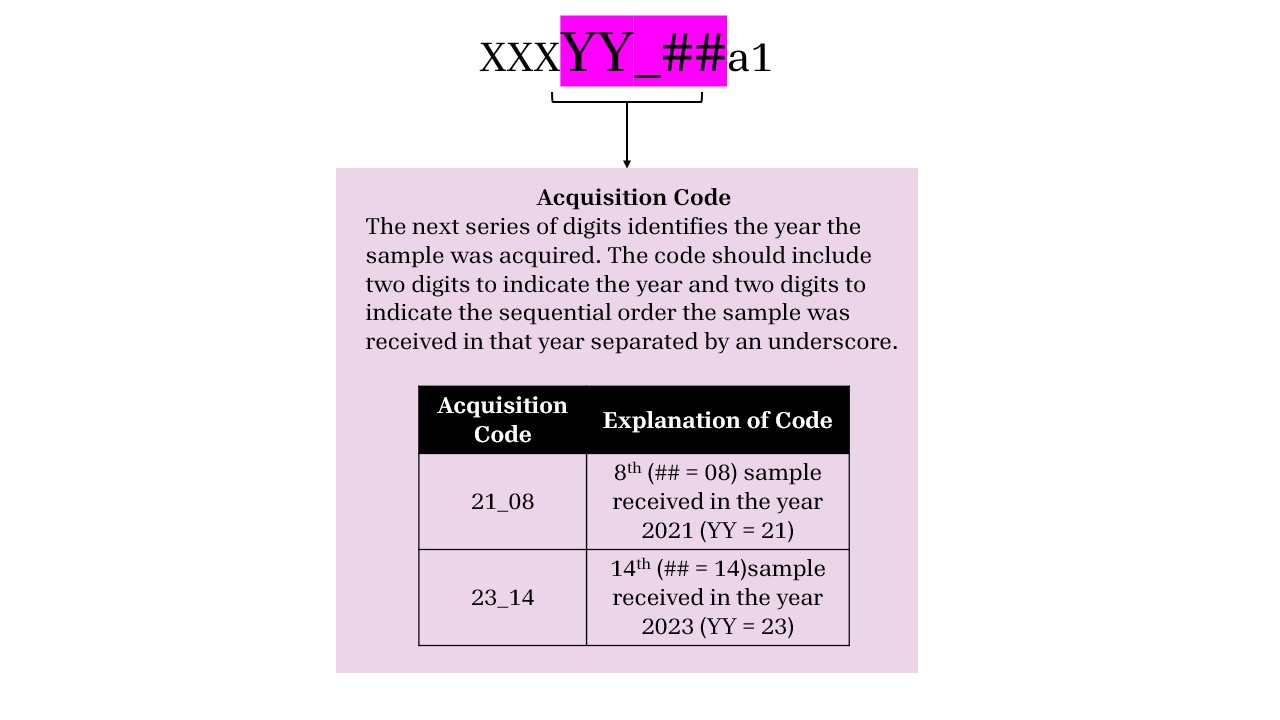
\includegraphics[width=1\linewidth]{figures/Slide3.jpg}
    \caption{Acquisition code description for sample naming convention.}
    \label{fig:nameAcq}
\end{figure}

\begin{figure}
    \centering
    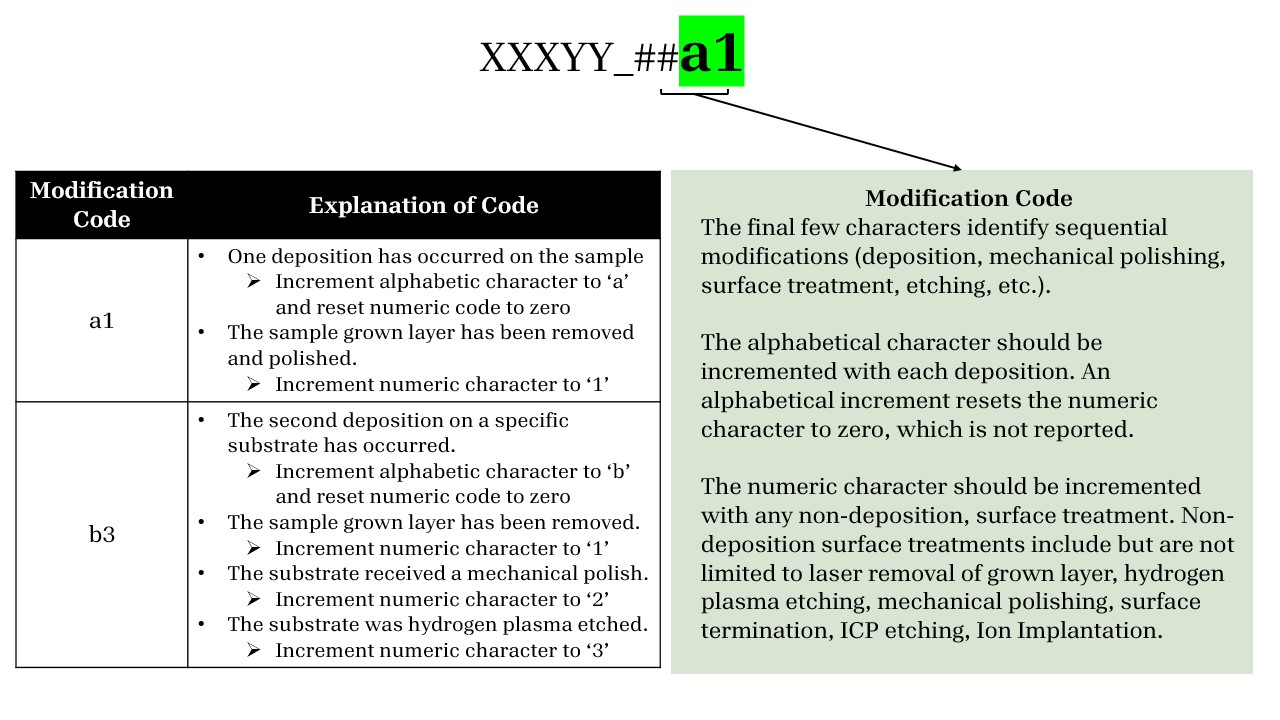
\includegraphics[width=1\linewidth]{figures/Slide4.jpg}
    \caption{Modification code description for sample naming convention.}
    \label{fig:nameMod}
\end{figure}

\begin{figure}
    \centering
    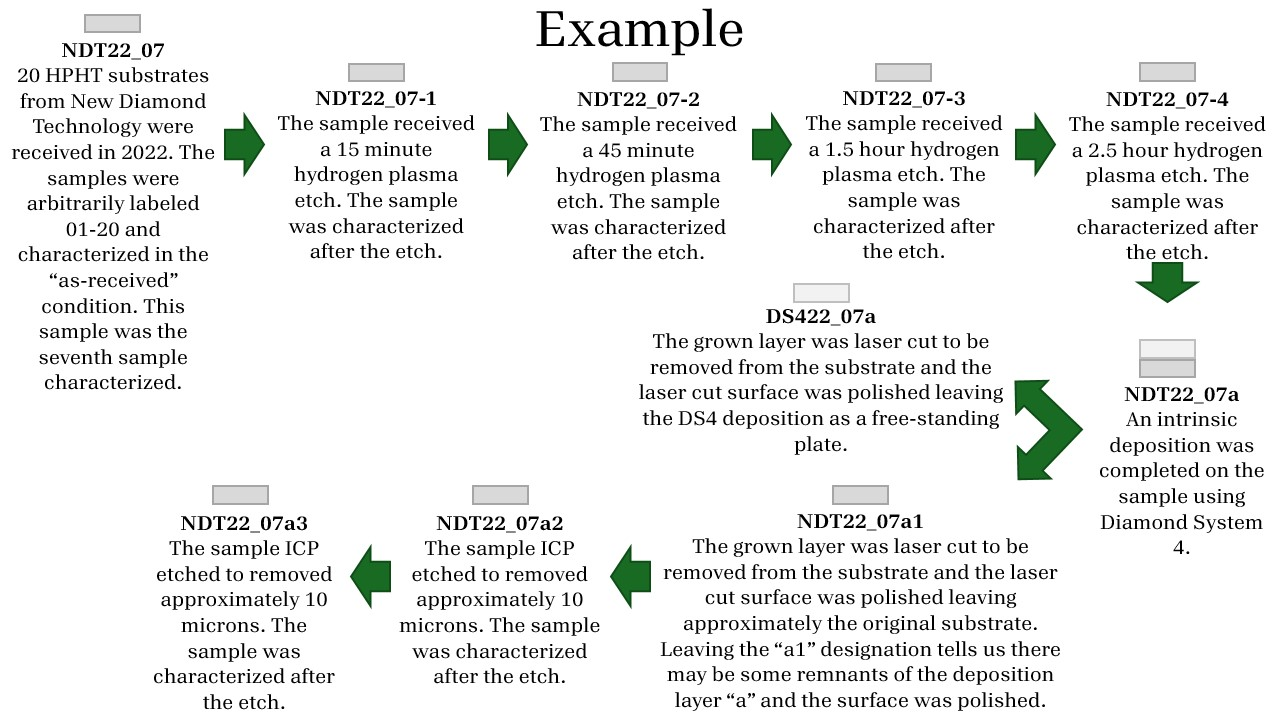
\includegraphics[width=1\linewidth]{figures/Slide6.jpg}
    \caption{Graphical example of naming convention implementation.}
    \label{fig:nameEx}
\end{figure}

%% To include several appendices, remove the only the "%"
%% in front of "\appendix".

%% In either cast to start your first appendix, which will be labeled
%% as Appendix A, just type \chapter{<appendix 1 name>}
%% and enter the text of the appendix as you would a chapter.

\end{doublespace}

%%%%%% Bibliography %%%%%
%% A bibliography is required. By default it is called, "Bibliography"
%% You may use �Literature Cited�, �Works Cited� or �References� 
%% instead of �Bibliography� if that is the convention in your discipline. 
%% To do so, place your choice in the empty argument 
%% of the following command and remove the "%".
\renewcommand{\bibname}{REFERENCES}


\bibliographystyle{unsrt}
\bibliography{references} %references in references.bib BibTeX file

% \ap
%% The bibliography may be made using BibTeX.
%% To do so the necessary commands must be entered in the 
%% preamble and here.
%% If the Bibliography is made from scratch,
%% remove the "%" in front of "\begin{thebibliography}{???}"
%% replacing the ??? with the appropriate entry and 
%% remove the "%" in front of "\end{thebibliography}"
% \begin{thebibliography}{???}
%% Enter the bibliography here.
% \end{thebibliography}
%% In either case, the bibliography is automatically entered
%% in the Table of Contents.
\end{document}